
\chapter{Projekt systemu}
\thispagestyle{chapterBeginStyle}

W tym rozdziale przedstawiony zostanie dokładny projekt systemu, jest on podzielony na kilka podrozdziałów. \textbf{Grupy użytkowników} oraz \textbf{Przypadki użycia} opisują szczegółowo, do czego i przez kogo będzie mogła zostać uzyta implementowana platforma. Sekcje \textbf{Diagramy aktywności} i \textbf{Diagramy sekwencji} pokazują, w jaki sposób udało się osiągnąć bardziej skomplikowane cele określone za pomocą przypadków użycia, niektóre funkcjonalności w zależności od ich charakterystyki zostaną przedstawione na diagramach aktywności - te dotyczące programisty ze względu na bardziej skomplikowane algorytmy, oraz na diagramach sekwecji - te bardziej nastawione na funkcjonalności biznesowe.

W kolejnych sekcjach znajdą się \textbf{Diagramy klas} oraz \textbf{Projekt bazy danych}. W pierwszej opisane zostaną klasy, które musiały zostać stworzne do implementacji procesów zdefiniowanych w wcześniejszych podrozdziałach, odpowiednio w drugiej znajdą się schematy bazy danych podzielone ze względu na funkcjonalności.

\section{Grupy użytkowników}
We frameworku możemy zdefiniować 3 grupy użytkowników, którzy będą korzystać z jego udogodnień. \textbf{Programista} jest to użytkownik frameworka, który implementuje swój sklep z pomocą narzędzi dostarczonych przez opisywany system. \textbf{Administrator} to ktoś, zajmujący się backofficową\footnote{backoffice - w systemach e-commerce panel do obsługi i utrzymania sklepu} obsługą sklepu - obsługa reklamacji. \textbf{Klient} jest to końcowy klient sklepu, który przegląda katalog i dokonuje zakupów. 

Warto zazanaczyć w tym momencie, że tematem pracy jest zaimplementowanie frameworka, co wskazuje na to, że funkcjonalności będą skupione głównie na programiście, rola administratora i klienta oraz przypadki użycia z nimi powiązane są jedynie zmienną w implementowanym systemie. Oznacza to nic innego, że rola administratora (i rzeczy, które może zrobić), są uzależnione od konfiguracji i dodadków systemu. Głównym celem jest to, aby stworzyć narzędzie dzięki, któremu możliwości administratora i klienta są ograniczone jedynie \textit{fantazją} programisty. Założenie to bardzo dobrze ilustruje następujący przykład:
\begin{example}
	Załóżmy, że implementujemy sklep internetowy, korzystając z opisywanego frameworka. Nasz pracodawca życzy sobie aby w sklepie pojawił się również blok z artykułami, którymi będzie można zarządzać w panelu administracyjnym. Normalnie proces implementacji takiej funkcjonalności wiązałby się z przygotowaniem modelu w bazie danych i pełnej jego obsługi, również ze strony front-endowej. Z użyciem frameworka proces można skrócić do zaimplementowania modelu i paru prostych koment aby wygenerować mechanizm do manipulacji stworzonym modelem - w przykładzie blogiem wraz z artykułami. 
\end{example}

\section{Przypadki użycia}
Jak zostało zdefiniowane w poprzednim punkcie, w pracy przewidziano 3 grupy użytkowników. W zamyśle framework jest narzędziem dla programisty, jednak w systemie został zaimplementowany szereg rozwiązań gotowych do wykorzystania dla końcowych użytkowników, dlatego diagramy przypadków użycia zostały podzielone na trzy klasy: 
\begin{itemize}
	\item przypadki użycia Programisty 
	\item przypadki użycia Użytkownika Administracyjnego potencjalnego serwisu e-commerce, opartego na opisywanym Frameworku
	\item przypadki użycia użytkownika końcowego, czyli Klienta
\end{itemize}
Na rysunku \ref{useCaseProgrammer} zostały przedstawione najważniejsze przypadki użycia frameworku. Programista ma swobodny dostęp do rozszerzania encji, w szczególności klasy Produkt, która ma wyjatkowo strategiczne znaczenie w systemach e-commerce. Dodatkowo ma możliwość uczynienia niestandardowych pól wyszukiwalnymi przez klienta. Sytuacja została zobrazowana na poniższym przykładzie.
\begin{example}
	Załóżmy, że mamy niestandardowe pole proste (String) w encji klasyfikowanej przez twórców ewentualnego sklepu związanego z opisywanym frameworkiem jako finalna encja nadająca się do sprzedaży. Niech nazywa się \texttt{MyProduct extends Product} z polem \texttt{myCustomField}. Jedyne co w tej sytuacji musimy zrobić aby system mógł wyciągnąć wartość tego pola z encji (o której de facto nie wie) to wpisać do tabeli zawierającej indeksowane cechy produktu nazwę danego pola, system za pomocą refleksji\footnote{\textit{refleksja} ( eng. reflection) -- udogodnienie w języku Java, pozwalające na wyświetlenie i manipulacje właściwościami klasy. Więcej w sekcji \textbf{słowniczek}.} wyekstaktuje wartość pola z encji.    


Dodane przez Programistę encje są obsługiwane przez framework, dodatkowo po dodaniu specjalnej adnotacji\footnote{adnotacja -- używane w języku Java od wersji 1.7, najczęściej służą do określania dodatkowych właściwości pól bądź klas} nad nią, może być zarządzana w uniwersalnym panelu administracyjnym. Osoba zajmująca się implementacją sklepu opartego o opisywaną platformę może uruchomić dowolną \textit{(skończoną)} ilość instancji Apache Solr, czyli bazy danych noSQL, służącej do obsługiwania zapytań związanych z katalogiem produktowym (skalowalność pionowa tylko tej części aplikacji, która tego potrzebuje). W odniesieniu do przypadku użycia \textit{Nadpisanie mechanizmu wyszukiwania} z rysunku \ref{useCaseProgrammer} serwisy są oparte na interfejsach, zapewniając Programiście możliwość nadpisania jego logiki zgodnie z zasadami polimorfizmu. 
\end{example}
\begin{figure}
\begin{center}
	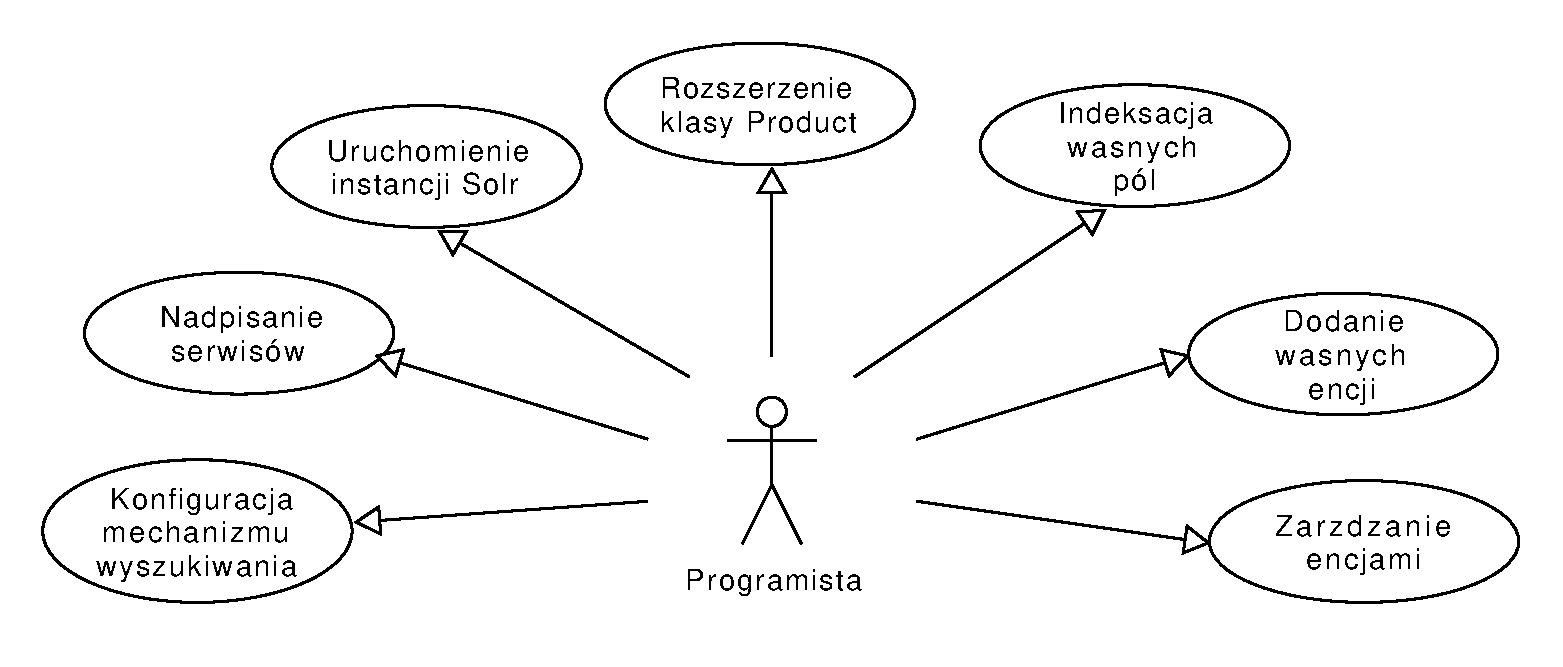
\includegraphics[width=1\textwidth]{ucdev.pdf}
\end{center}
\caption{{\color{black}Diagram przypadków użycia związany z Programistą.}} \label{useCaseProgrammer}
\end{figure}
\begin{figure}
	\begin{center}
		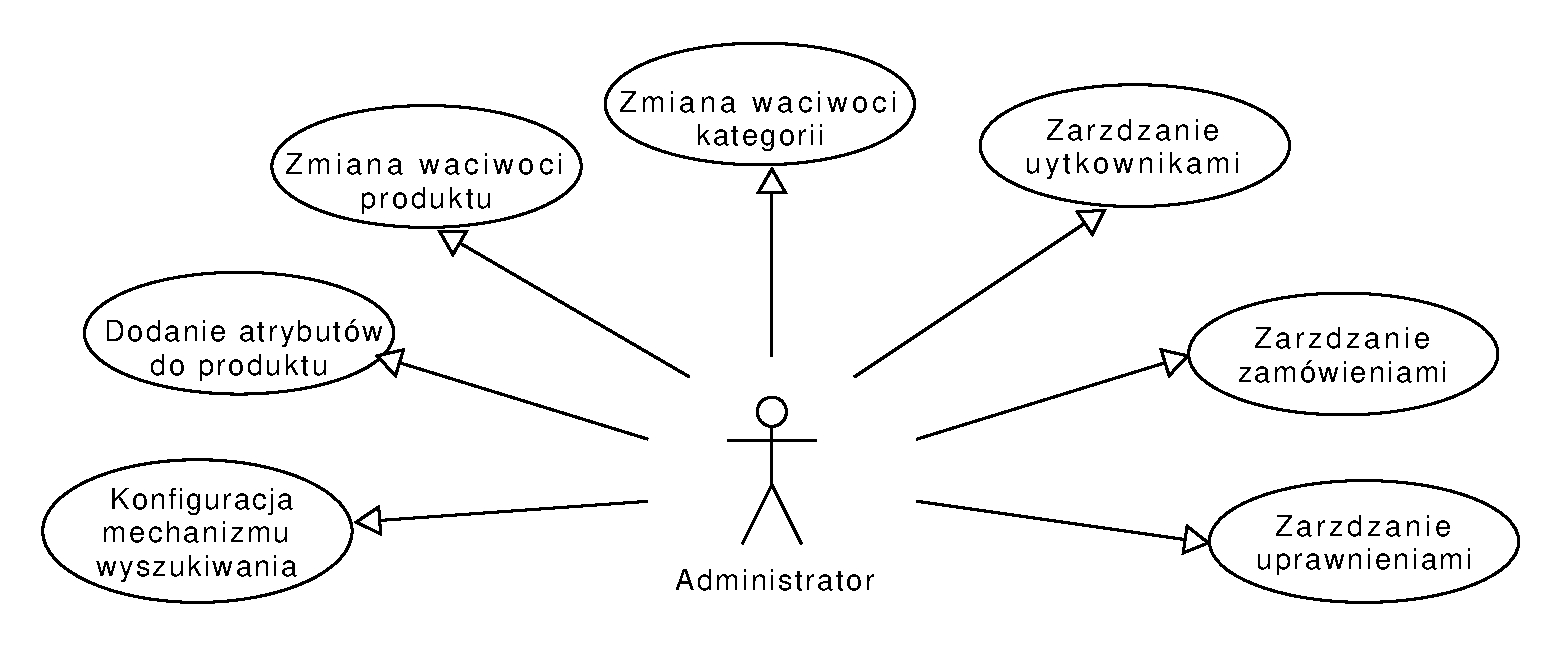
\includegraphics[width=1\textwidth]{ucadmin.pdf}
	\end{center}
	\caption{{\color{black}Diagram przypadków użycia związany z Administratorem ewentualniego systemu.}} \label{useCaseAdmin}
\end{figure}
Rysunek \ref{useCaseAdmin} przedstawia przypadki użycia z punktu widzenia Administratora potencjalnego systemu. Z punktu widzenia platformy jest to również klient, gdyż framework zakłada, że nie ma on wiedzy technicznej i nie potrafi programować. Podobnie jak programista, może konfigurować mechanizm wyszukiwania, jednak bardziej wysokopoziomowo, np. deklaracja używanych facetów. Panel administracyjny zakłada zarządanie najważniejszymi encjami: produkt, kategoria, użytkownik, zamówienie, uprawnienie i parę innych, zdefiniowanych dokładniej w podrozdziale \textbf{Diagramy bazy danych}.

Diagram na rysunku \ref{useCaseCustomer} dotyczy przypadków użycia elementów frameworku przez końcowego użytkownika. Są to klasyczne funkcjonalności tradycyjnego sklepu internetowego. \textit{Wyszukanie produktu} zostało zaprojektowane, tak aby możliwy był również do zaimplementowania mechanizm podpowiedzi i podświetlania. Apache Solr udostępnia taką funkcjonalność. \textit{Reklamacja} dotyczy opisanego w rozdziale \textbf{Analiza problemu} kłopotu z archwizacją produktu, został on rozwiązany prostym mechanizmem wersjonowania. 
\begin{figure}
	\begin{center}
		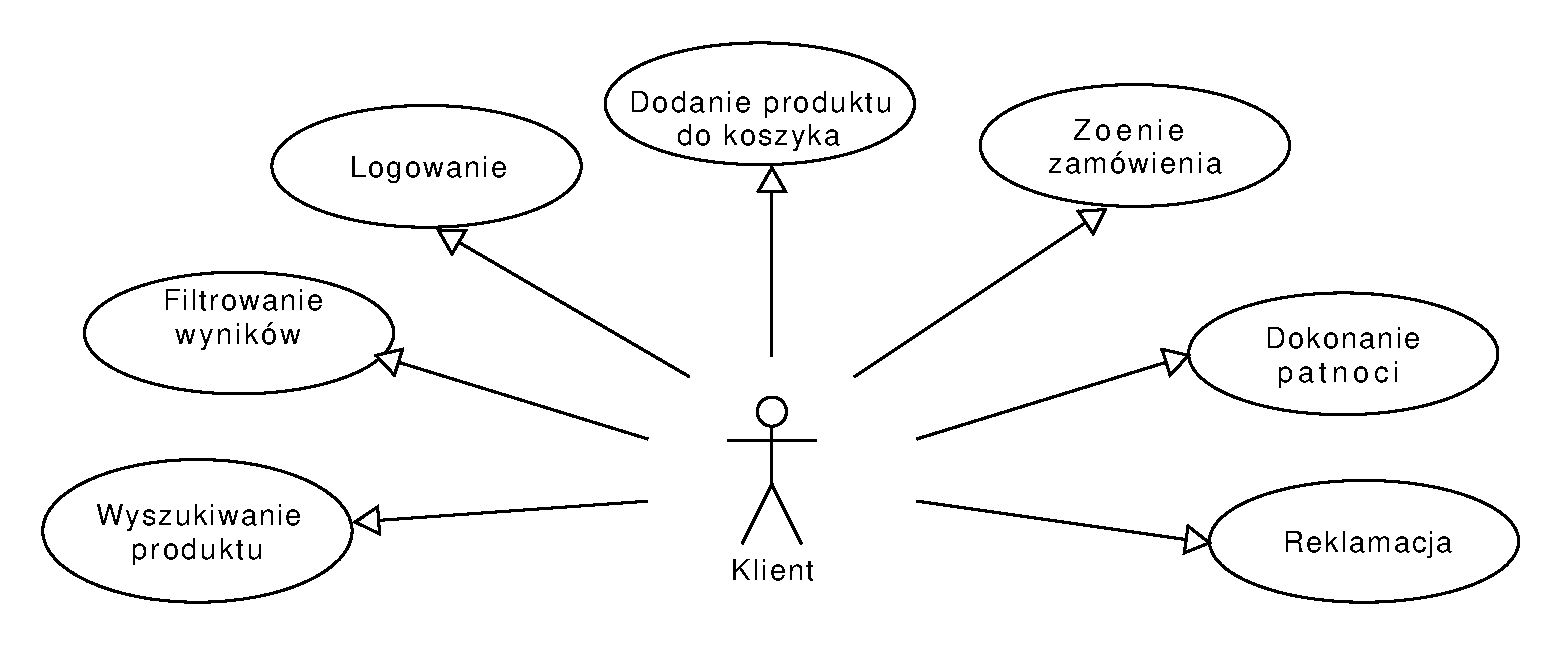
\includegraphics[width=1\textwidth]{uccustomer.pdf}
	\end{center}
	\caption{{\color{black}Diagram przypadków użycia związany z Klientem końcowym ewentualniego systemu.}} \label{useCaseCustomer}
\end{figure}

Diagramy typu \textit{use-case} ściśle wiążą się z wymaganiami funkcjonalnymi systemu. Jest wiadome, że można je również sklasyfikować pod względem aktorów występujących w systemie, dlatego też powiązania przypadków użycia z wymaganiami funkcjonalnymi zostały umieszczone na diagramie z rysunku \ref{wymtoUC}. Na diagram należy patrzeć poziomo, po zapoznaniu się z legendą. Wymagania są w nieprzypadkowej kolejności, są ustawione od lewej do prawej. Im bardziej na prawo, tym wymaganie jest bardziej biznesowe, im bardziej na lewo -- dotyczy rdzeniowych elementów platformy. Warto zauważyć zależność, że im dalej patrzymy na diagram, tym więcej niebieskich i żółtych \textit{use case'ów} -- tych zarezerowowanych dla Administracji i Klientów rozwiązania e-commerce. Natomiast im bardziej na lewo tym więcej czerwonego, czyli przypadków przemyślanych dla Programisty.
\begin{figure}
	\begin{center}
		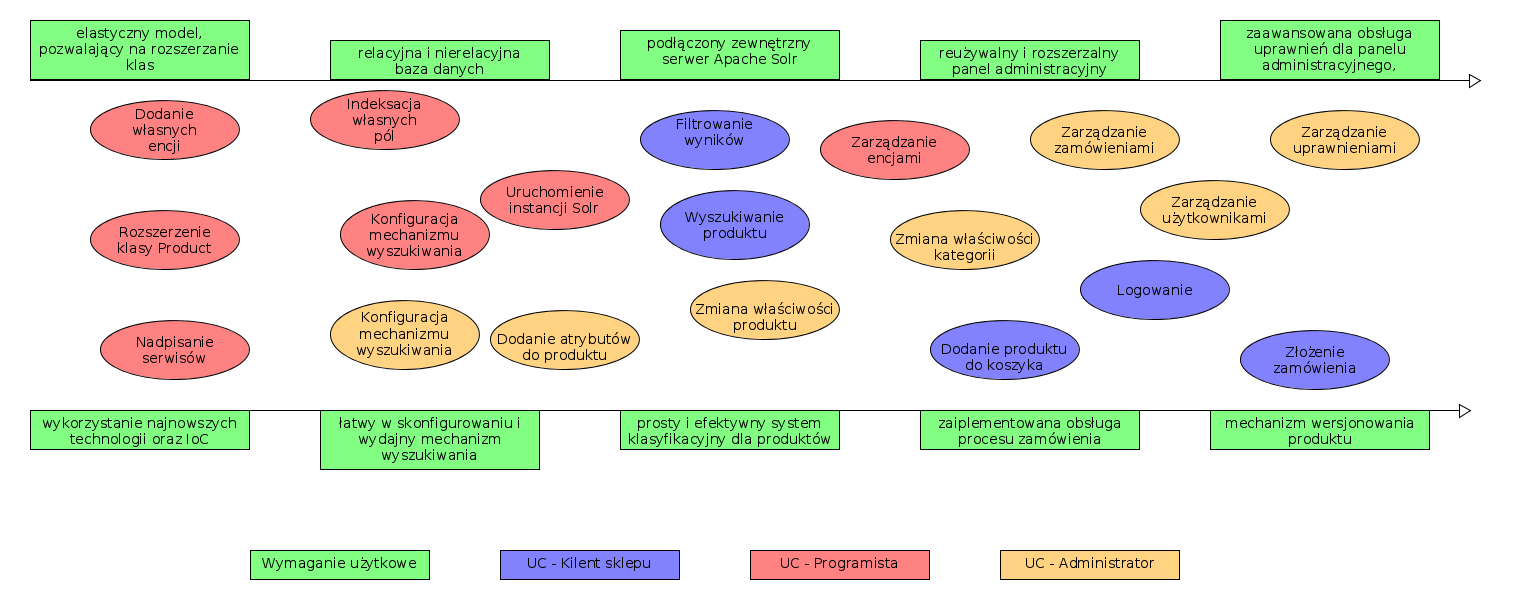
\includegraphics[angle=270,scale=0.4]{wymToUC.png}
	\end{center}
	\caption{{\color{black}Diagram przypadków użycia związany z wymaganiami funkcjonalnymi}} \label{wymtoUC}
\end{figure}

Jak zostało wspomniane wcześniej w sekcji \textbf{Grupy użytkowników i założenia}, framework jest narzędziem głównie dla programisty, to on zdecyduje co ma się znajdować w finalnym systemie, dlatego w niniejszym podrozdziale zostaną rozwinięte przypadki użycia dla programisty związane z obsługą i oprogramowywaniem dynamicznych elementów platformy. Jest to odpowiedź na najtrudniejsze z wymagań, czyli \textbf{elastyczny model, pozwalający na rozszerzenie klas} oraz \textbf{reużywalny i rozszerzalny panel administracyjny}.
\subsection{Dynamiczna tabela encyjna}
Dynamiczna tabela encyjna jest autorskim rozwiązaniem, służącym do wylistowywania dowolnych encji związanych z systemem w panelu administracyjnym, wiążą się z nim przpadki użycia z rysunku \ref{dynEntTabUC}
\begin{figure}[H]
	\begin{center}
		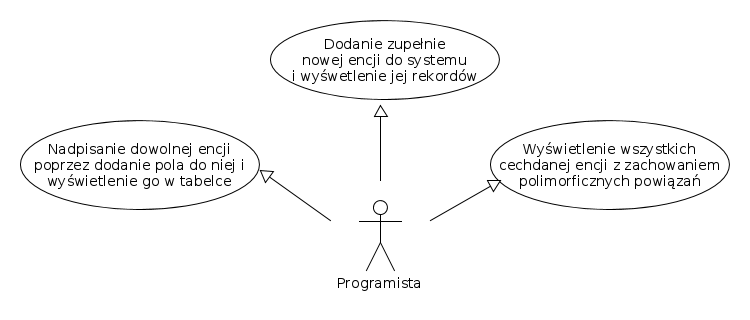
\includegraphics[scale=0.5]{dynEntTabUC.png}
	\end{center}
	\caption{{\color{black}Diagram przypadków użycia związany z dynamiczą tabelą encyjną}} \label{dynEntTabUC}
\end{figure}

\subsection{Dynamiczny formularz encyjny}
Dynamiczny formularz encyjny to kolejne autorskie rozwiązanie, służące do dodawania edycji i wyświetlania szczegółów encji związanych z systemem w panelu administracyjnym, wiążą się z nim przpadki użycia z rysunku \ref{dynEntFormUC}
\begin{figure}[H]
	\begin{center}
		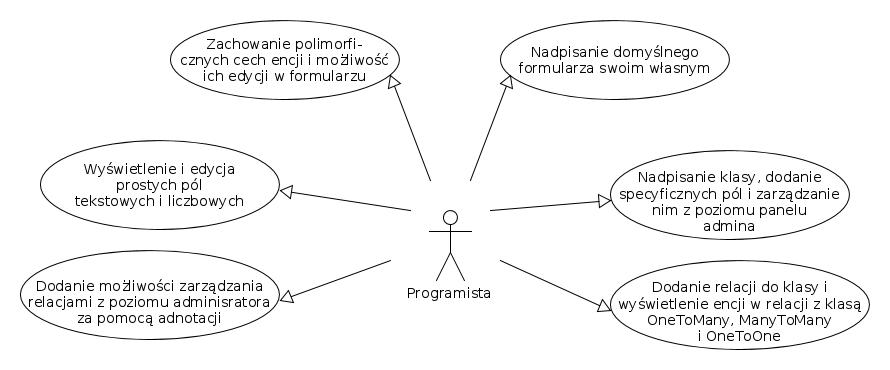
\includegraphics[scale=0.5]{dynEntFormUC.png}
	\end{center}
	\caption{{\color{black}Diagram przypadków użycia związany z dynamicznym formularzem encyjnym}} \label{dynEntFormUC}
\end{figure}

\subsection{Manipulacja produktem}
Produkt w implementowanym systemie jest to encja bardzo dynamiczna, łatwo konfigurowalna. Wiążą się z nim przypadki użycia znajdujące się na rysunku \ref{manipProd}
\begin{figure}[H]
	\begin{center}
		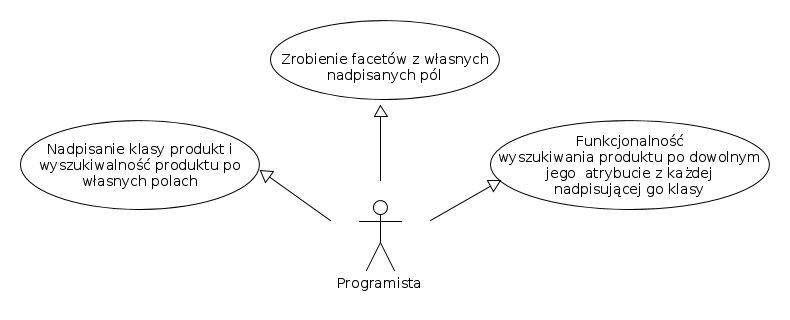
\includegraphics[scale=0.5]{manipProd.png}
	\end{center}
	\caption{{\color{black}Diagram przypadków użycia związany z dynamicznym formularzem encyjnym}} \label{manipProd}
\end{figure}

\section{Diagramy aktywności}
W tej sekcji zostały przedstawione diagramy aktywności dla najbardziej skomplikowanych logicznie elementów systemu. Dynamiczna tabela i formularz opisany w poprzednim punkcie wymagają skomplikowanych operacji aby mogły pozostać ogólne i elastyczne na tyle ile być muszą. Znaczy to, że powinny obsługiwać zmiany w modelu wywołane przez osoby trzecie - \textbf{programistów}. W niniejszym podrozdziale przedstawiono działanie algorytów stojących za dynamicznymi elementami platformy.

\subsection{Wyszukiwanie cech produktu}
Ta sekcja odnosi się do podrozdziału \textbf{Manipulacja produktem}. Wytłumaczono tutaj jak osiągnięto założoną elastyczność przy konfigurowaniu encji reprezentującej produkt w sklepie. 

Każdy Produkt w systemie jest indeksowany, oznacza to że z relacyjnej bazy danych, wraz ze swoimi wszystkimi atrybutami trafia do nierelacyjnych dokumentów na osobnym serwerze, aby odciążyć aplikacje w razie dużego ruchu. Zebranie wszystkich atrybutów produktów to skomplikowane zadanie, gdyż jego cechy mogą być ukryte w następujących miejscach: 
\begin{itemize}
	\item atrybuty dziedziczone po atrybutach klasyfikacyjnych kategorii, w której się znajduje
	\item atrybuty dziedziczone po wszystkich przodkach swojej kategorii
	\item własne pola i pola wszystkich klas, które nadpisały Produkt 
\end{itemize}  

Zadanie to wymaga zejścia do poziomu refleksji w Javie, jednak ten temat został poruszony później. Wyszukiwaniem wszystkich atrybutów obsługuje algorytm, którego diagram aktywności został umieszczony na rysunku \ref{diagramaktywIndeks}

Pierwszym krokiem jest znalezienie wszystkich produktów, co nie jest również oczywistym zadaniem, gdyż nie jest wiadome jaką klasę ma finalny produkt, mógł zostać nadpisany przez programistę, który w swojej klasie zdefiniował pewne pola, które również muszą zostać uwzględnione przy indeksacji produktów. Po znalezieniu \textit{klasy sufitowej} (czyli najwyższej w abstrakcji) mamy pewność, że wszystkie niestandardowe pola znajdą się w obiekcie pobranym przez nas z bazy danych. Z bazy danych muszą zostać również pobrane pola zadeklarowane jako te, które są wyszukiwalne w sklepie (oczywiste jest, że powinno się mieć wybór, które pola z produktu trafią do sklepu, a które nie). Mając te dwie rzeczy, jest możliwe wyciągnąć z obiektu, którego klasa nie jest znana wszystkie interesujące nas pola. Wszystkie wyciągnięte wartości następnie trafiają do dokumentu. Nie jest to jeszcze koniec, gdyż zostają nam jeszcze do wyciągnięcia cechy produktu z systemu klasyfikacyjnego, zostało to zrealizowane algorytmem przejścia po drzewie oraz zapytaniem bazodanowym. Wszystkie cechy produktu są dodawane do listy dokumentów (jeden dokument - jeden produkt) i są wysyłane na serwer Apache Solr. Przykład skąd mogą pochodzić cechy produktu został umieszczone na rysunku \ref{cechyProd}.
\begin{figure}
	\begin{center}
		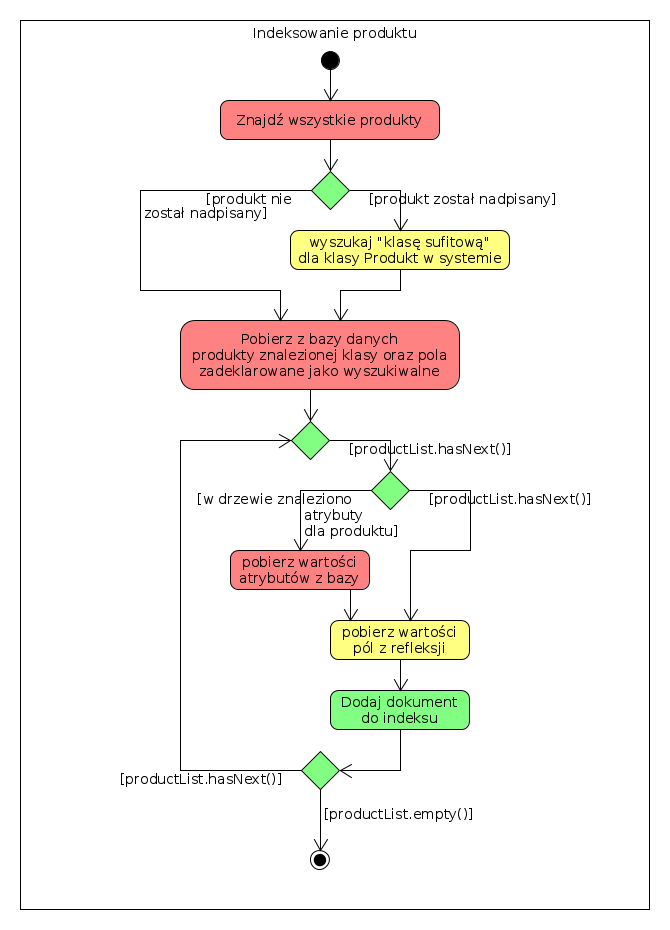
\includegraphics[scale=0.5]{diagramaktywIndeks.png}
	\end{center}
	\caption{{\color{black}Diagram aktywności opisujący algorytm znajodwania wszystkich atrybutów produktu}} \label{diagramaktywIndeks}
\end{figure}
\begin{figure}
	\begin{center}
		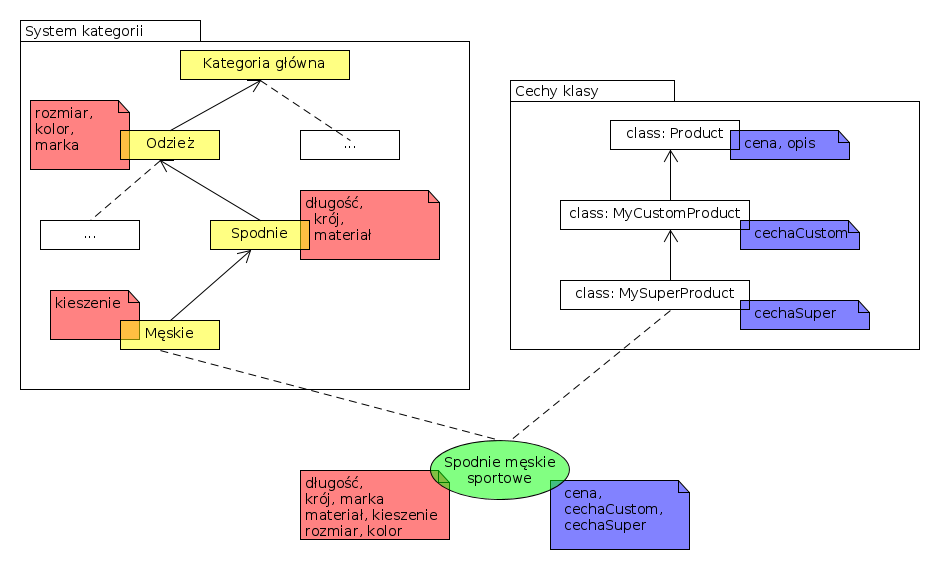
\includegraphics[scale=0.5]{cechyProd.png}
	\end{center}
	\caption{{\color{black}Diagram przykładowy skąd mogą pochodzić cechy produktu}} \label{cechyProd}
\end{figure}

\subsection{Konstrukcja zapytania dynamicznego Apache Solr}
Na diagramach use case zostały opisane możliwości konfiguracji mechanizmu wyszukującego. Zdefiniowane wymagania zostały zrealizowane za pomocą konstrukcji dynamicznego zapytania. W prostych słowach chodzi tu o kwerendę zwracającą produkty przy wyszukiwaniu. Wykres na rysunku \ref{konsDynZapy} przedstawia algorytm tworzący te zapytania. Pierwszy etap widoczny na rysunku nasuwa podejrzenie, że w bazie danych musi istnieć tabela z wylistowanymi polami, które będą wyszukiwalne w sklepie, jest to jak najbardziej trafne przypuszczenie. Dodatkowo w tabeli zostały umieszczone dodatkowe ustawienia dla pól wyszukiwania, aby mechanizm mógł być w pełni konfigurowalny. 
\begin{figure}
	\begin{center}
		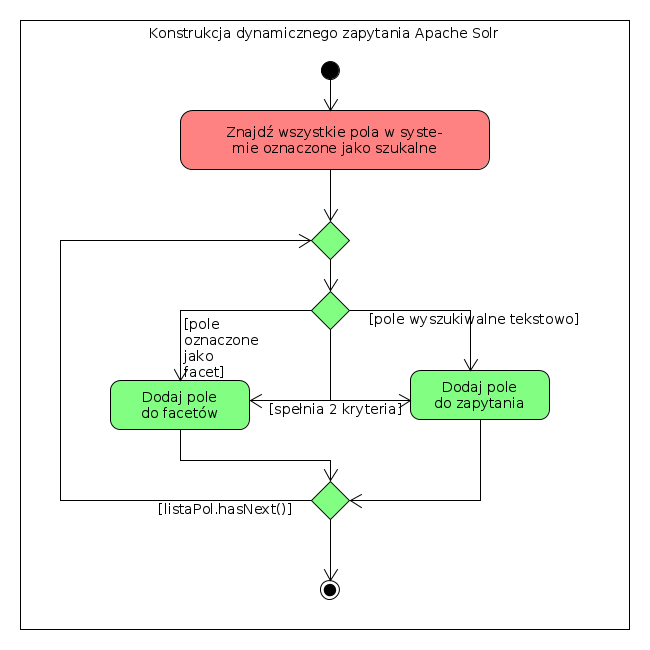
\includegraphics[scale=0.5]{konsDynZapy.png}
	\end{center}
	\caption{{\color{black}Diagram przedstawiający algorytm kostrukcji dynamicznego zapytania Apache Solr}} \label{konsDynZapy}
\end{figure}
\subsection{Konstrukcja dynamicznej tabeli encyjnej}
Dynamiczna tabela encyjna opisana w poprzednim podrozdziale, jest wbrew pozorom zadaniem analogicznym do wyciągania cech z produktu. Ułatwieniem jest to, że w tabeli nie uwzględnia się atrybutów z systemu klasyfikacyjnego, gdyż dotyczy on tylko produktów, niestety utrudnieniem jest to, że nie jest wiadome jakie klasy dokładnie powinny być wyświetlone w tabelach. Jedyne co jest dane to tabela konfiguracyjna z kodami klas, które mają zostać wyświetlone w panelu administracyjnym. Proces został opisany na diagramie z rysunku \ref{konsTabEnc} 

Najpierw szukane są encje z rodzaju podanego we wspomnianej tablei, następnie refleksją wyciąga się jej pola zaadnotowane przez programistę jako te, które chce wyświetlić w tabeli jako nagłówki (adnotacja \texttt{@AdminVisible(tableVisible=true)}). Ze znalezionej listy obiektów pobiera się wartości pól, które znajdują się w nagłówkach.
\begin{figure}
	\begin{center}
		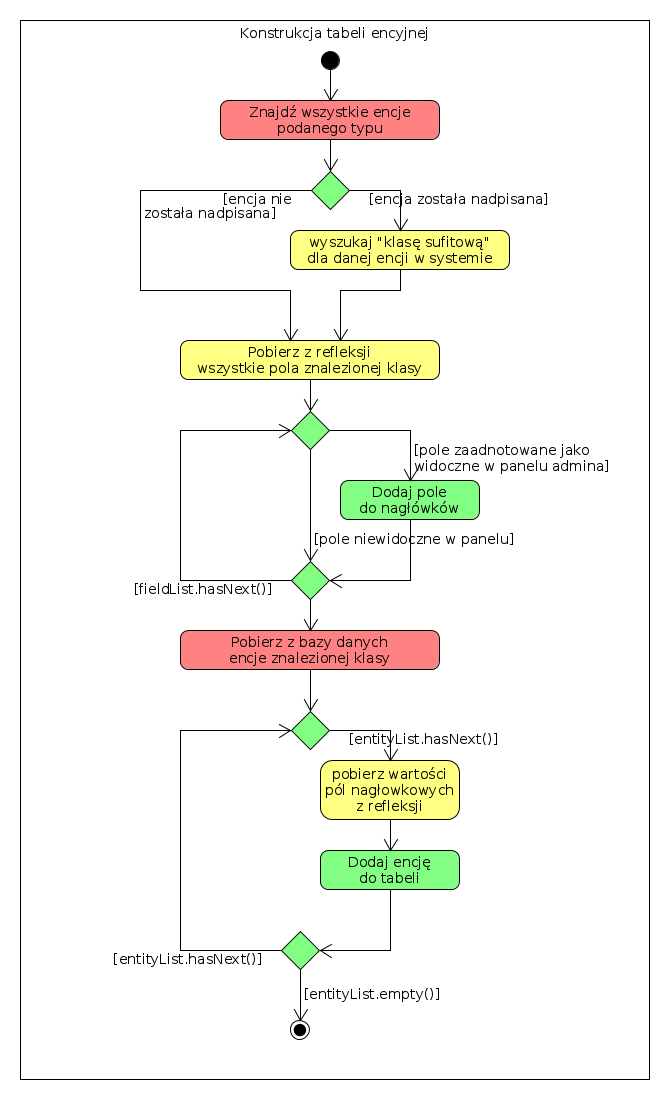
\includegraphics[scale=0.5]{konsTabEnc.png}
	\end{center}
	\caption{{\color{black}Diagram aktywności opisujący algorytm wyszukujący cechy encji uwzględnianych w tabeli.}} \label{konsTabEnc}
\end{figure}

\newpage
\subsection{Konstrukcja dynamicznego formularza encyjnego} \label{s_konDynForm}
Odbywa się to na bardzo podobnej zasadzie, jak konstrukcja tabeli. Jednak poza polami prostymi zaadnotowanymi jako widzialne w panelu administracyjnym, problem stanowią relacje, które trzeba wyświetlić. Aby zachować rozszerzalność platformie zastosowane zostały tu mechanizmy z dwóch poprzednich przykładów. Po znalezieniu listy pól danej klasy, następuje tu jeszcze sklasyfikowanie ich względem tego, czy są to relacje czy nie. Wiadome jest, że relacji nie można przedstawić w postaci pola tekstowego, dlatego potrzebujemy wtedy ręcznie doczytać kolekcję w relacji z encją, której detale są wyświetlane. Wszystkie kolekcje są w systemie kolekcjami leniwymi (ze względu na performance), dlatego przy manipulacji encją jej duże elementy takie jak kolekcje są doczytywane dopiero w moemencie ich użycia(ponieważ wymagają joinów, a wiadome jest że join to iloczyn kartezjański, oczywiście odpowiednio napisany nie będzie dokładnie tym samym jednak to i tak duże obciążenie). W zwykłej sytuacji framework Hibernate doczytałby sam tę kolekcję, jednak przy tak dużej ogólności rozwiązania nie jest to możliwe, gdyż na poziomie dynamicznego formularza mówimy o \texttt{AbstractEntity}\footnote{AbstractEntity - klasa w systemie reprezentująca najbardziej podstawową encję, jej cechy to id oraz kod}, o której właściwie w ogóle nie ma informacji, więc Hibernate nie jest \textit{świadomy} manipulacji i nie doczyta jej kolekcji nawet będąc w sesji. To przysporzyło wiele kłopotów, jednak problem został rozwiązany ręcznym doczytaniem kolekcji za pomocą Criteria API\footnote{Criteria API - API do komunikacji z bazą danych, zgodne se standardem JPA, używane do bardziej zaawansowanych i niestandardowych operacji}. Schemat algorytmu rozwiązującego problem został umieszczony na rysunku \ref{konsFormEnc}.

\begin{figure}
	\begin{center}
		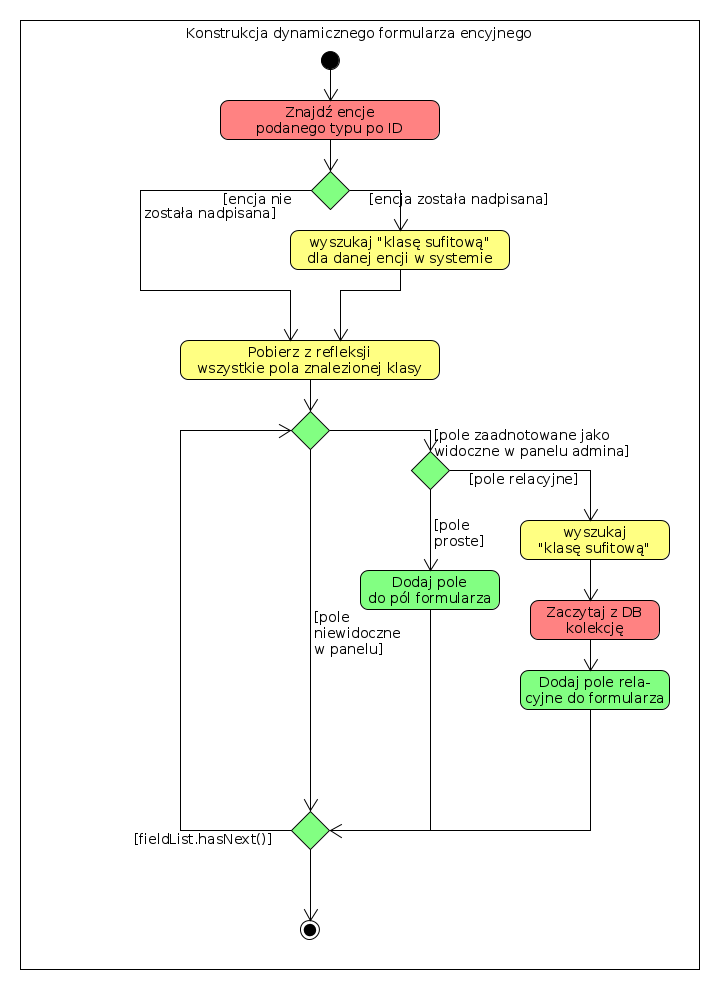
\includegraphics[scale=0.5]{konsFormEnc.png}
	\end{center}
	\caption{{\color{black}Diagram aktywności opisujący algorytm wyszukujący cechy encji uwzględnianych w tabeli.}} \label{konsFormEnc}
\end{figure}

\subsection{Podsumowanie diagramów aktywności}
Diagramy aktywności i zaprezentowane rozwiązania w nich pokrywają pewne przypadki użycia, w tej sekcji zostanie podkreślone jak przedstawione algorytmy spełniają zdefiniowane use case'y.

Patrząc na sekcję \textbf{Wyszukiwanie cech produktu} i \textbf{Konstrukcja zapytania dynamicznego Apache Solr} zostały zrealizowane następujące przypadki użycia:
\begin{itemize}
	\item Programisty: 
	\subitem Rozszerzenie klasy produkt
	\subitem Konfiguracja mechanizmu wyszukiwania
	\subitem Indeksacja własnych pól
	\item Administratora:
	\subitem Konfiguracja mechanizmu wyszukiwania
	\subitem Dodanie atrybutów do produktu
	\subitem Zmiana właściwości produktu
	\item Klienta sklepu
	\subitem Wyszukiwanie produktu
	\subitem Firtrowanie wyników
\end{itemize}

Sekcja \textbf{Konstrukcja dynamiczniej tabeli encyjnej} i \textbf{Konstrukcja dynamicznego formularza encyjnego} pokryły następujące przypadki użycia:
\begin{itemize}
	\item Programisty: 
	\subitem Konfiguracja panelu administracyjnego
	\subitem Dodanie własnych encji
	\subitem Zarządzanie encjami
	\item Administratora:
	\subitem Zmiana właściwości kategorii
	\subitem Zarządzanie użytkownikami 
	\subitem Zarządzanie zamówieniami
	\subitem Zarządzanie uprawnieniami
\end{itemize}

W podrozdziale opisującym przypadki użycia opisano również przypadki w sekcjach o dynamicznym formularzu, tabeli i manipulacji produktem, oczywiste jest, że wspomniane użycia bezpośrednio wiążą się z opisanymi komponentami.

Realizacja przypadków użycia, których nie mogły pokryć algorytmy opisane w niniejszym podrozdziale ze względu na swoje biznesowe pochodzenie, zostaną opisane na diagramach sekwencji. 

\section{Diagramy sekwencji}

W tej sekcji zostały przedstawione diagramy sekwencji dla poszczególnych elementów systemu, mają one razem z diagramami aktywności zrealizować wszystkie przypadki użycia. Diakramy sekwencji dobrze oddają sens funkcjonalności biznesowych i właśnie ich dotyczy ta sekcja. 

\subsection{Zmiana właściwości dowolnej encji}
W każdym systemie bazodanowym, konieczna jest manipulacja encjami. We wcześniejszych rozdziałach zostało wprowadzone pojęcie dynamicznych tabel i formularzy edycyjnych. Z punktu widzenia bazy danych, nie ma dużego znaczenia jaka encja jest edytowana, zarówno Produkt jak i Kategoria to jedynie zbiór krotek w tabeli relacyjnej, dlatego właśnie zdecydowano się na generyczny mechanizm modyfikacji encji. W prostych słowach, w systemie nie ma osobnych formularzy edycyjnych dla poszczególnych encji, są one generowane na podstawie kodu Javowego. 

Funkcjonalność zmiany właściwości dowolnej encji zostanie omówiona na przykładzie zmiany nazwy produktu, ale jak już wyżej wspomniałem, ten sam mechanizm działa w dowolnej encji, która może być modyfikowana przez framework. Po zalogowaniu się i wyświetleniu menu, administrator wybiera dowolny produkt, po czym zmienia dane pole w formularzu edycji i następnie zapisuje produkt. Diagram \ref{zmianaWlEncji} przedstawia cały proces. Najważniejsze etapy to 5 oraz od 8 do 13, to one odpowiedzialne są za elastyczność systemu - każda encja jest modyfikowana w ten sam sposób - generycznie, przez refleksję. W tym miejscu widać główny cel i zamysł pracy: system jest siadomy tego jaki obiekt edytuje, dlatego może mieć dostęp do jego właściwości (9. findPolimorficFieldsOf) - metoda ta zwraca wszystkie możliwe pola dla danego obiektu, właśnie dlatego, gdy programista nadpisze jakąś klasę, która jest używana w systemie, nic się nie stanie gdyż framework będzie w stanie wyciągnąć z obiektu każde nowe pole. Mechanizm ten zastosowany jest również we wszystkich kluczowych funkcjonalnościach, co skutkuje bardzo elastycznym modelem.
\begin{figure}
	\begin{center}
		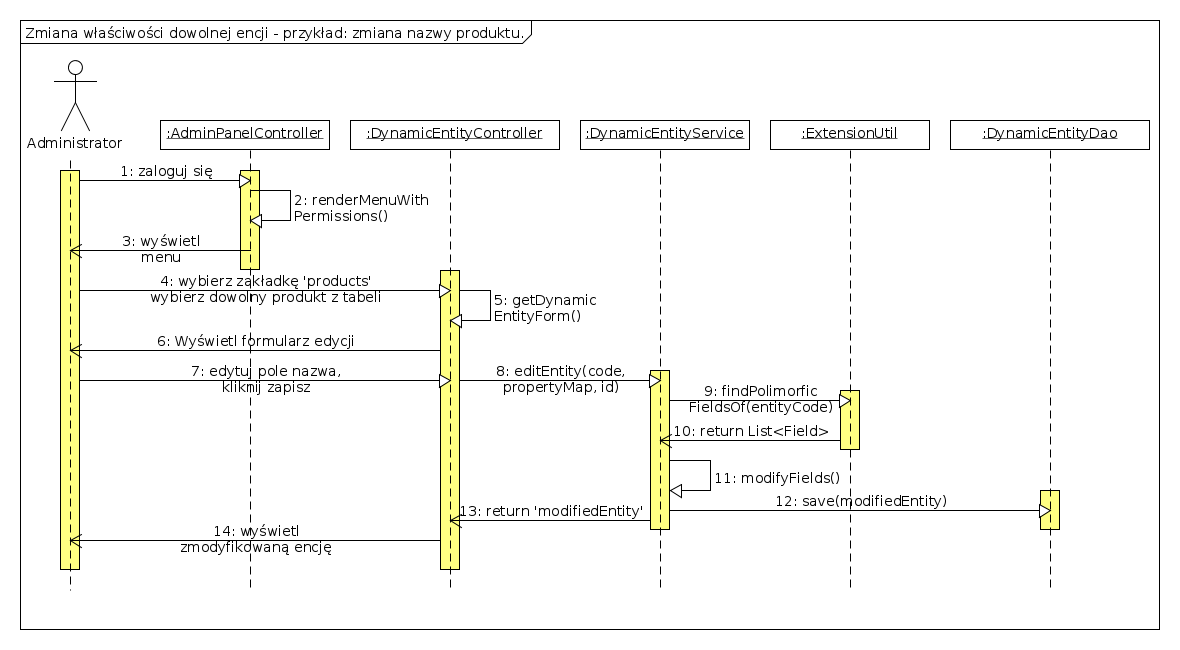
\includegraphics[scale=0.4]{zmianaWlEncji.png}
	\end{center}
	\caption{{\color{black}Diagram sekwencji opisujący opiisujący zmianę właściwości dowolnej encji na przykładzie produktu.}} \label{zmianaWlEncji}
\end{figure}

\subsection{Modyfikacja dowolnej relacji encji}
Dynamiczny formularz encyjny omówiony na diagramach aktywności zawiera również pola relacyjne, rysunek \ref{zmianaWRel} przedstawia diakram sekwencji zmiany w relacji dowolnej encji na przykładzie dodania dziecka do kategorii. Okazuje się być dużym problemem dla frameworka, gdyż modyfikowany jest obiekt pewnej klasy i tylko na tej podstawie potrzeba określić jakie ma relacje i co więcej, wyciągnąć je z bazy danych. Problem został rozwiązany poprzez wprowadzenie do systemu dodatkowych parametrów adnotacji \texttt{@AdminVisible} takich jak nazwa klasy \texttt{className} i mapowanie relacji \texttt{mappedBy} - punkt 5 na rysunku \ref{zmianaWRel}, następnie dla wszystkich encji relacyjnych zostaje zbudowana dynamiczna tabela - tylko że wewnątrz formularza edycyjnego (pkt. 6 do 8). Następnie po kliknięciu \textit{add} przy tabelce z relacją, pobierana jest lista możliwych do przypisania encji i w przypadku kliknięcia na dany rekord, zostaje on wprowadzony w relację z edytowaną encją. Kolejne punkty odpowiadają za elastyczność rozwiązania, czyli ponownie (jaj w poprzednich funkcjonalnościach), dla każdej znalezionej encji należy znaleźć klasę sufitową i to na jej podstawie wyciągać pola i tworzyć powiązania. Całość jest przedstawiona w formie pól tekstowych, checkboxów i tabelek z relacjami.
 \begin{figure}
 	\begin{center}
 		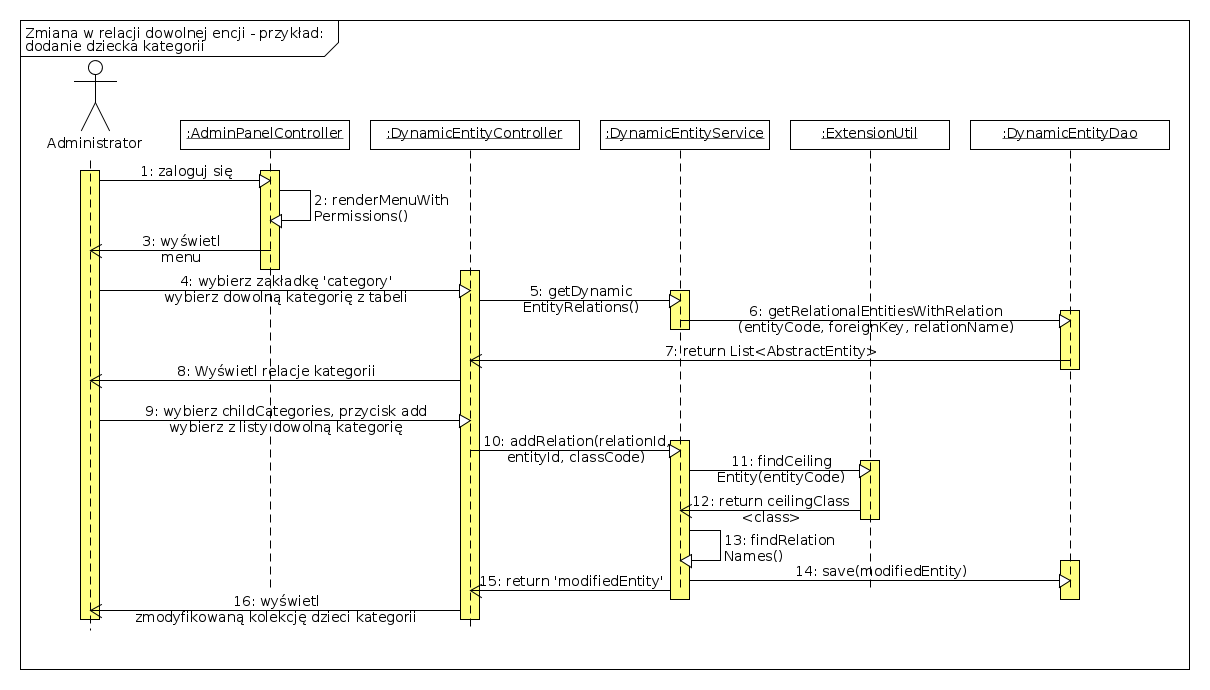
\includegraphics[scale=0.4]{zmianaWRel.png}
 	\end{center}
 	\caption{{\color{black}Diagram sekwencji opisujący opiisujący zmianę właściwości dowolnej encji na przykładzie produktu.}} \label{zmianaWRel}
 \end{figure}

\subsection{Dodanie dowolnej encji na przykładzie atrybutu klasyfikacyjnego}
Ta ważna część frameworku zostanie przedstawiona na podstawie dodawania facetu - czyli atrybutu, po którym można filtrować produkt. Tak jak w powyższych sekcjach, nie ma dużego znaczenia jaką encję dodajemy - generyczny formularz i mechanizm uzupełniania pól w obiekcie danej klasy jest taki sam dla wszystkich encji w systemie. Dzięki diagramowi sekwecji z rysunku \ref{dodanieFacetu} można zobaczyć jak dodać atrybut do produktu, który będzie wyszukiwalny, a zarazem zobaczyć jak w systemie persystowane są nowe obiekty. Tym razem refleksja została użyta do przepisania wartości z formularza do obiektu (punkty 8 do 12) oraz do znalezienia najwyższej w hierarchii klasy modyfikowanej encji (pkt 5). 

Jak zostało już wspomniane, każdy atrybut może mieć wartości, które powinien przyjmować, np. \textit{rodzaj podszewki: skórzana/gumowa/materiałowa}. Dlatego do atrybutu klasyfikacyjnego możliwe jest zdefiniowane jego przyjmowanych wartości, dzieje się to w dokładnie ten sam sposób, jak na rysunku \ref{dodanieFacetu}, jedynie encja z \texttt{CategoryFeature} (atrybut klasyfikacyjny) zmienia się na \texttt{CategoryFeatureValue}. Po dodaniu możliwych wartości dla stworzonego atrybutu, należy je do niego przypisać w sposób opisany w sekcji \textbf{Modyfikacja dowolnej relacji encji} na diagramie z rysunku \ref{zmianaWRel} oraz dodać atrybut z możliwymi wartościami do relacji kategorii (w formularzu edycji dla kategorii rys. \ref{zmianaWlEncji} i \ref{zmianaWRel}). Atrybut zostanie uwzględniony w wynikach wyszukiwania opisanych w podrozdziale \textbf{Wyszukiwanie prduktu}. Aby rozjaśnić rozważania, został przytoczony przykład \ref{przyklAtrubyt}.
\begin{example} 
	Załóżmy, że w mamy kategorię obuwie, chcielibyśmy aby każdy produkt w wynikach wyszukiwania w sklepie był możliwy do odfiltrowania na podstawie rodzaju podszewki. W tym celu dodajemy atrybut klasyfikacyjny Podszewka z zaznaczeniem, że ma być to facet (filtr). Dodajemy 3 wartości: skórzana/gumowa/materiałowa. Przypisujemy możliwe wartości do atrybutu, sam atrybut do kategorii obuwie, od tej pory w formularzu edycyjnym produktu, który znajdzie się w kategorii obuwie, znajdziemy pole rodzaj podszewki. Co więcej gdy więcej niż jeden znaleziony przy wyszukiwaniu w sklepie produkt będzie miał zdefiniowany dla siebie ten atrybut, to pojawi się on (atrybut) jako przycisk do odfiltrowania.  
	\label{przyklAtrubyt}
\end{example}
 
  \begin{figure}
 	\begin{center}
 		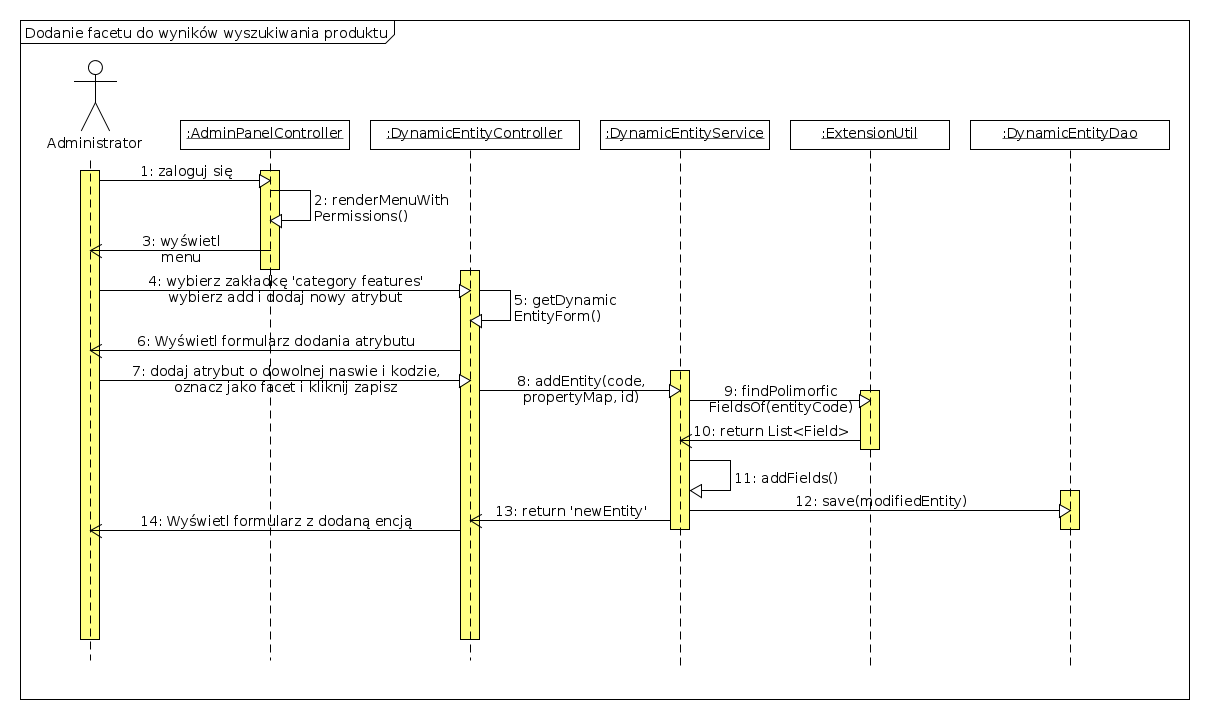
\includegraphics[scale=0.4]{dodanieFacetu.png}
 	\end{center}
 	\caption{{\color{black}Diagram sekwencji opisujący dodanie dowolnej encji na przykładzie atrybutu klasyfikacyjnego.}} \label{dodanieFacetu}
 \end{figure}

\subsection{Wyszukiwanie produktu}
Proces wyszukiwania produktu został ujęty na diagramie z rysunku \ref{wyszukiwanieProdSekw}. Aby przedstawić to jak najbardziej obrazowo, w procesie uczestniczą trzy komponenty: frameworkowy kontroler wyszukiwania, serwer Solr, który przechowuje produkty w płaskiej strukturze i baza danych relacyjna, która przechowuje pola i włąsciwości produktu podlegające mechnizmowi wyszukiwania. Na początku z bazy danych wciągane są właściwości i wszystkie zmienne, więc to czy dane pole ma być wyszukiwalne tekstowo, czy ma być filtrem (facetem). Następnie budowana jest dynamiczna kwerenda i wysyłana na serwer Apache Solr, który zwraca wyniki przetwarzane w punktach 10 do 12. Budowane są wtedy reprezentacje filtrów jak i samych wyników wyszukiwania, czyli produktów. 

Wart zauważenia jest region wykresu w ramce \textit{cached}, otóż jednym z postulatów frameworku było nie korzystanie z bazy danych relacyjnej przy wyszukiwaniu w katalogu produktowym (najbardziej obciążony fragment systemu), dlatego właściwości potrzebne do stworzenia kwerendy są pobierane raz, a później trzymane w pamięci cache (jest to mechanizm domyślnie dostarczany przez Hibernate, nie wymagał on implementacji). 
  \begin{figure}
	\begin{center}
		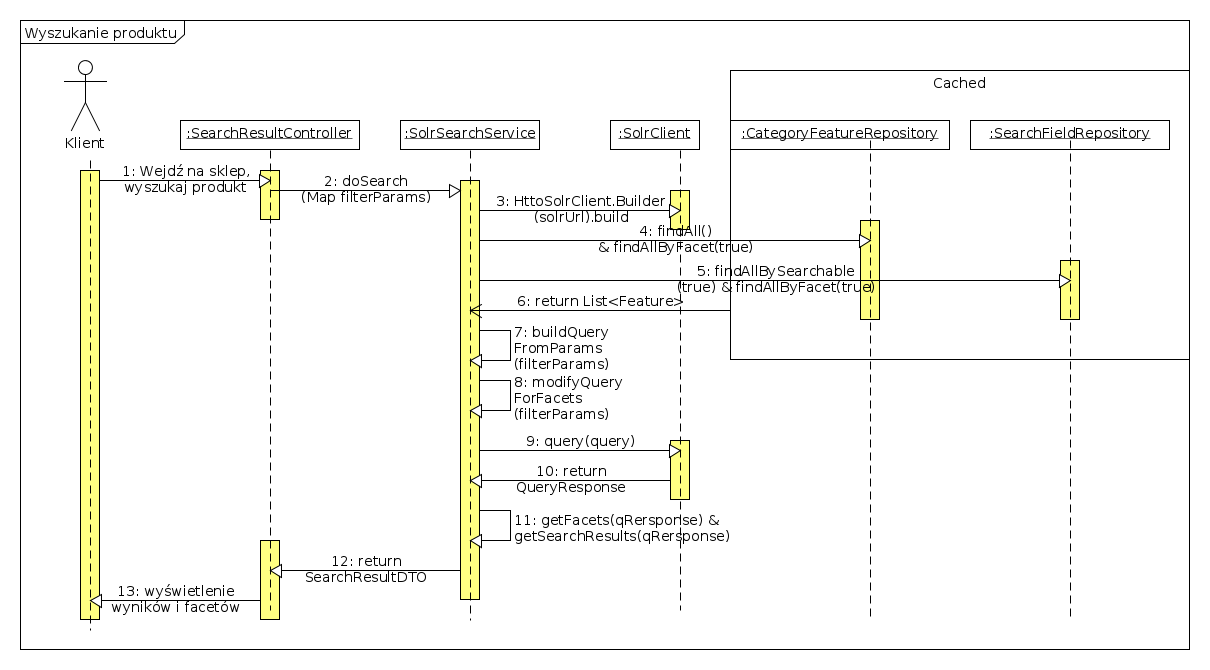
\includegraphics[scale=0.4]{wyszukanieProdSekw.png}
	\end{center}
	\caption{{\color{black}Diagram sekwencji opisujący proces wyszukiwania produktu.}} \label{wyszukiwanieProdSekw}
\end{figure}



\subsection{Proces zakupowy}
Proces zakupowy jest standardowym mechanizmem konicznym do przeprowadzenia transakcji, nie wymaga on szczególnej optymalizacji, ze względu na to, że nie jest to obciążona część platformy. Klient po wyszukaniu produktu może się zalogować i umieścić go w koszyku, a następnie zamówić produkty dodane do koszyka. Szczególnym rozwiązaniem dla frameworka jest stworzenie kopii produktu w tym momencie, aby klient w razie reklamacji miał się do czego odwołać, gdyż parametry produktu są bardzo dynamiczne i często się zmieniają, więc coś sprzedane 2 tygodnie wcześniej może być niemożliwe do odnalezienia po pewnym czasie. Funkcjonalność ta jest jedną z prostszych i nie wymaga dalszego opisu. Całość została umieszczona na diagramie z rysunku \ref{procZakup}
\begin{figure}
	\begin{center}
	%	\includegraphics[scale=0.4]{procZakup.png}
	\end{center}
	\caption{{\color{black}Diagram sekwencji opisujący proces zakupowy.}} \label{procZakup}
\end{figure}

\subsection{Proces reklamacji}
Proces reklamacji, ujęty na diagramie \ref{procRek} podobnie jak proces zakupowy, jest przykładowym procesem, który został zaimplementowany za pomocą modelu frameworka, oczywiście jest jego częścią, jednak nie wnosi dużej wartości do samej pracy. Został on zaimplementowany z powodu wspomnianego w rozdziale \textbf{Wymagania funkcjonalne}, we frameworkach e-commerce rzadko spotyka się takie funkcjonalności \textit{out of the box} dlatego jest to coś dodatkowego - rozszerzenie platformy.
\begin{figure}
	\begin{center}
	%	\includegraphics[scale=0.4]{procRek.png}
	\end{center}
	\caption{{\color{black}Diagram sekwencji opisujący proces zakupowy.}} \label{procRek}
\end{figure}

\newpage
\section{Diagramy klas}

Na podstawie wcześniejszych rozważań możliwe jest zdefiniowanie następujących części frameworku: 
\begin{itemize}
	\item system klasyfikacyjny i katalog produktowy
	\subitem model
	\subitem warstwa serwisowa systemu klasyfikacyjnego
	\item proces zamówienia i wersjonowania produktu
	\item dynamiczna obsługa modelu w panelu administracyjnym
	\subitem formularz encyjny
	\subitem tabela encyjna
	\subitem menu w panelu administracyjnym
	\item mechanizm indeksacji i wyszukiwania produktów
\end{itemize}
Diagramy klas zostaną podzielone ze względu na pochodzenie funkcjonalności zdefiniowane wyżej. 

\subsection{System klasyfikacyjny i katalog produktowy}

\subsubsection{Model systemu klasyfikacyjnego}
opis
\begin{figure}[H]
	\begin{center}
		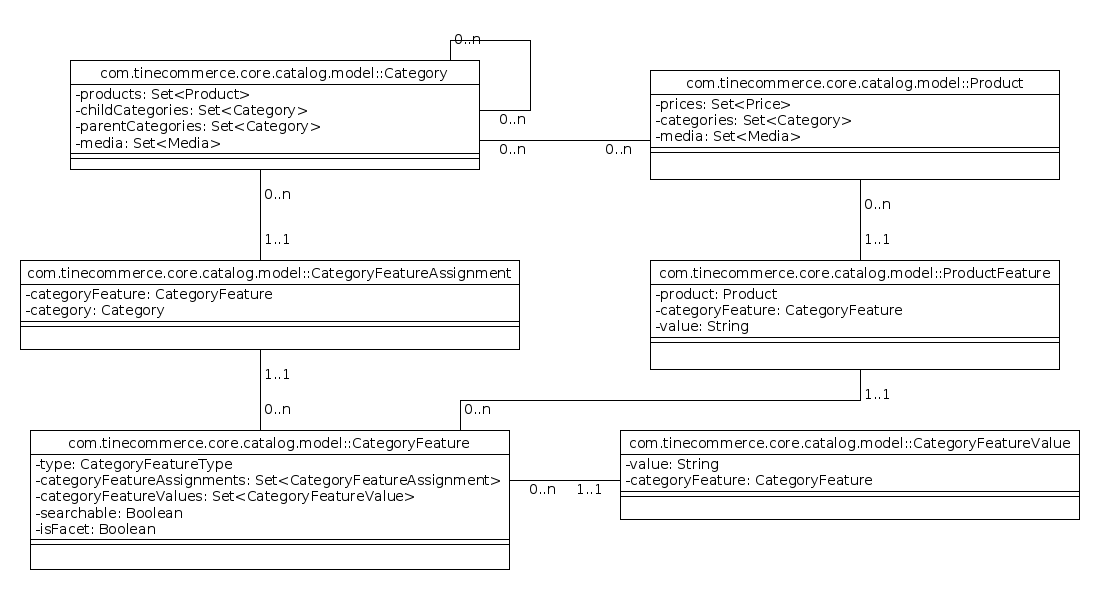
\includegraphics[scale=0.5,angle=270]{klasy_model_sysKlas.png}
	\end{center}
	\caption{{\color{black}Diagram klas systemu klasyfikacyjnego - model}} \label{klasy_model_sysKlas}
\end{figure}

\subsubsection{Warstwa serwisowa systemu klasyfikacyjnego}
opis
\begin{figure}[H]
	\begin{center}
		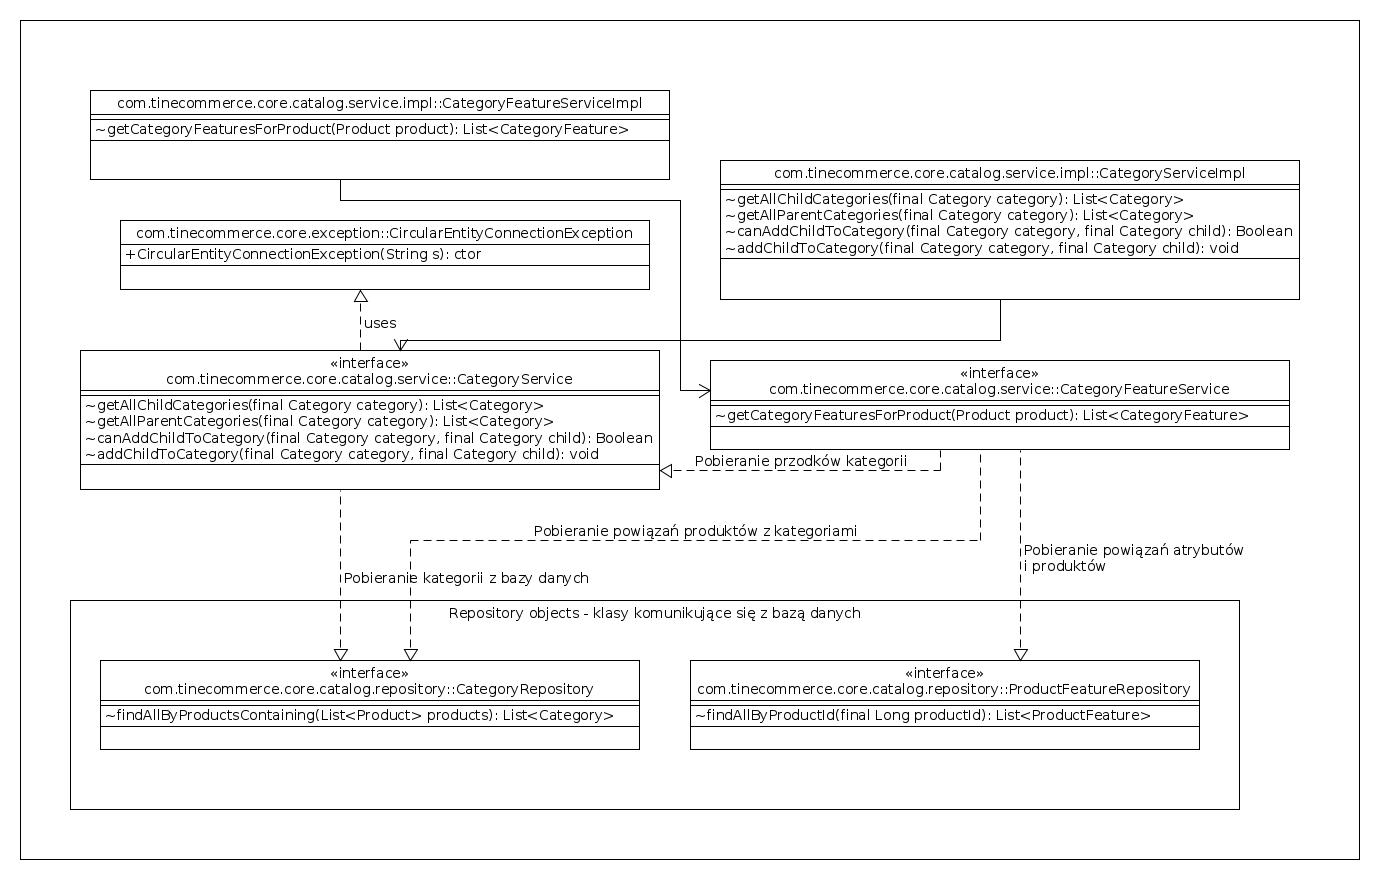
\includegraphics[scale=0.4,angle=270]{klasy_serwisy_sysKlas.png}
	\end{center}
	\caption{{\color{black}Diagram klas systemu klasyfikacyjnego - serwisy}} \label{klasy_serwisy_sysKlas}
\end{figure}

\subsubsection{Warstwa fasadowa systemu klasyfikacyjnego}
opis
\begin{figure}[H]
	\begin{center}
		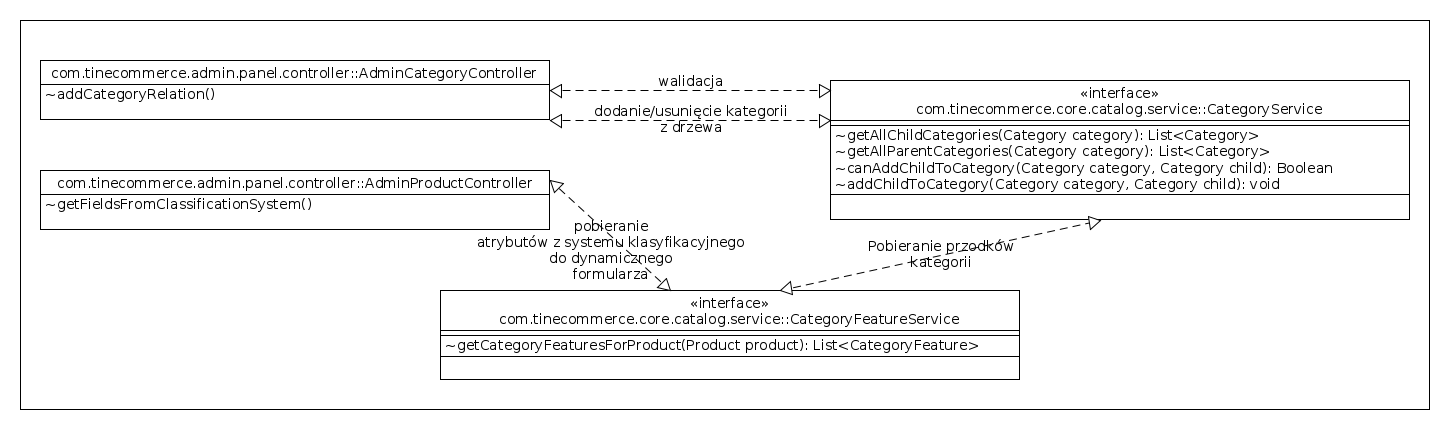
\includegraphics[scale=0.4,angle=270]{klasy_kontrolery_sysKlas.png}
	\end{center}
	\caption{{\color{black}Diagram klas systemu klasyfikacyjnego - fasada}} \label{klasy_kontrolery_sysKlas}
\end{figure}

\section{Projekt bazy danych}

W tej sekcji należy przedstawić projekt bazy danych. Należy omówić wycinek rzeczywistości i odpowiadające mu zidentyfikowane elementy systemu, których wartości będą podlegać utrwalaniu. Należy przedyskutować wybór typów danych dla atrybutów poszczególnych obiektów. Należy uzasadnić wybór platformy DBMS. Dla relacyjnych baz danych należy przedyskutować jej normalizację.

